\documentclass[11pt,a4paper]{article}
\usepackage[a4paper, margin=1.3in]{geometry}
\usepackage{mathtools}
\usepackage{fancyhdr}
\usepackage{mathrsfs}

\newcommand{\sheetNr}{13}

\pagestyle{fancy}
\fancyhf{}
\lhead{AI Planning}
\rhead{Exercise Sheet \sheetNr}
\lfoot{Axel Perschmann, Tarek Saier, \today}
\rfoot{Page \thepage\ of \pageref{lastpage}}
\renewcommand{\headrulewidth}{0.3pt}
\renewcommand{\footrulewidth}{0.3pt}
\setlength\parindent{0pt}
\newcommand{\h}[0]{\text{--}}

\begin{document}
\begin{center}
\Huge{\textbf{AI Planning}}\\
\LARGE{\textbf{Exercise Sheet \sheetNr}}
\end{center}
\vspace{2cm}
\begin{tabular}{ll}
Date: & \today\\
Students: & Axel Perschmann, Tarek Saier
\end{tabular}

\section*{Exercise 13.1}

\section*{Exercise 13.2}
(a)\\
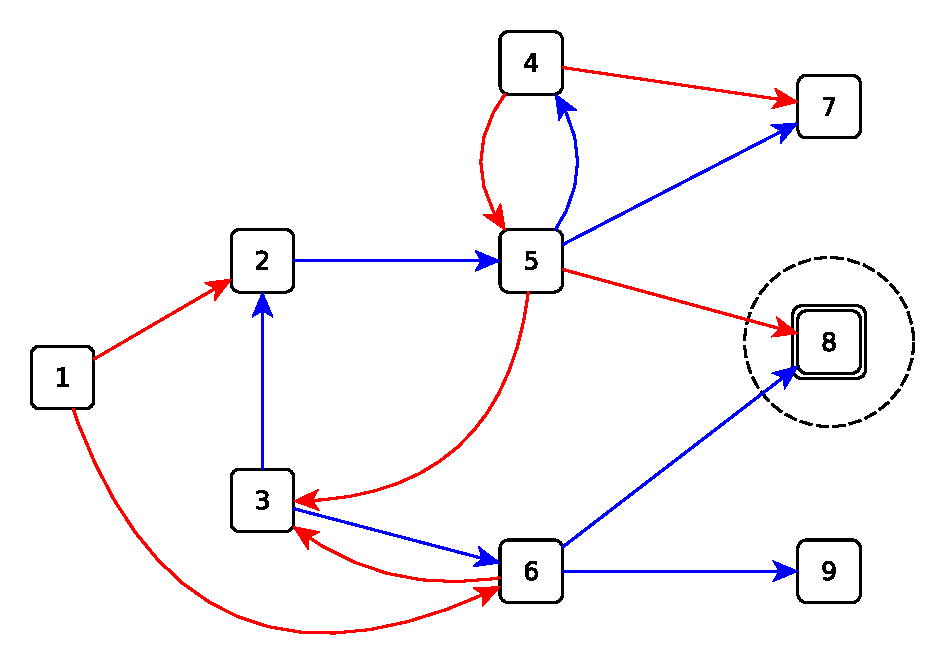
\includegraphics[scale=0.4]{13_2_0.pdf}\\
$C_0=S$, where $W_1=\{5,6\},W_2=\{1,2,3,4,5,6\}$\\
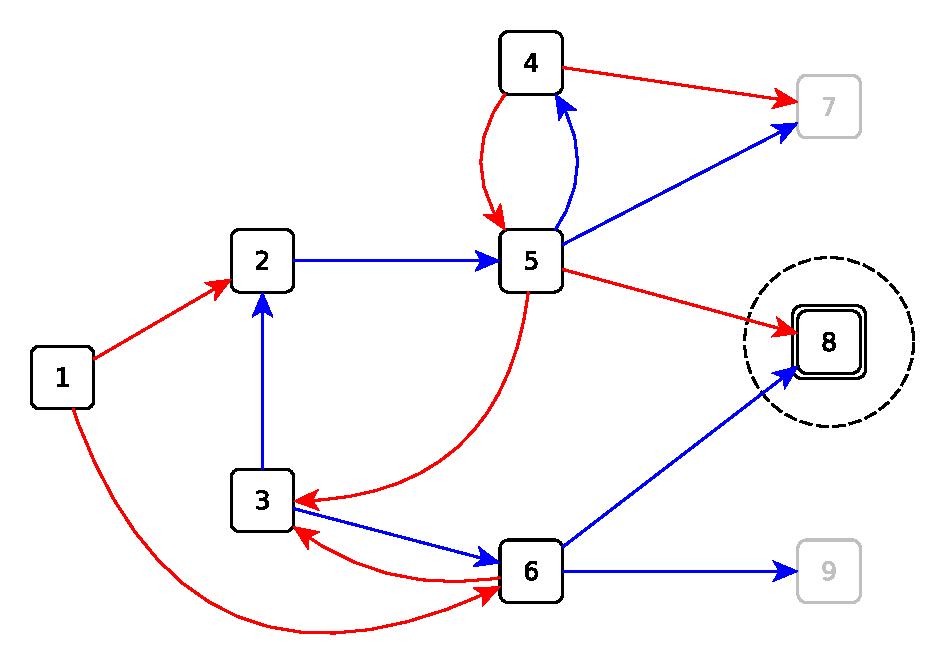
\includegraphics[scale=0.4]{13_2_1.pdf}\\
$C_1=\{1,2,3,4,5,6\}$, where $W_1=\{5\},W_2=\{2,5\},W_3=\{1,2,3,5\},W_4=\{1,2,3,5,6\}$\\
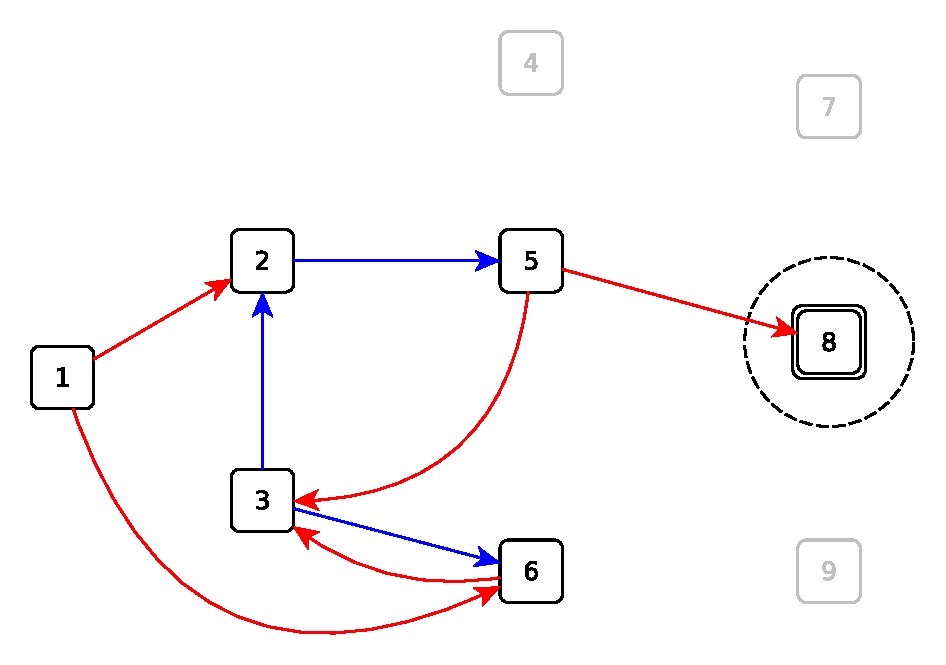
\includegraphics[scale=0.4]{13_2_2.pdf}\\
$\pi(s_1)=b,\pi(s_2)=a,\pi(s_3)=a,\pi(s_5)=b,\pi(s_t6)=b$
\\
(b) Let $o_l$ and $o_r$ denote the left and right arc of a nondeterministic operator (when looking in the direction their pointing in).\\
\\
\begin{tabular}{c|l|l|l|l}
\# & s & $\pi'$ & fail & $\pi$ \\
\hline
0 & & & $s_1$ & $\emptyset$ \\
1 & $s_1$ & $b_l,a,b_l$ & $s_3,s_6$ & $\{s_1\to b,s_2\to a,s_5\to b\}$ \\
2 & $s_3$ & $a_r,a_l$ & $s_6$ & $\{s_1\to b,s_2\to a,s_5\to b,s_3\to a,s_6\to a\}$ \\
3 & $s_6$ & $a_l$ & $s_9$ & $\{s_1\to b,s_2\to a,s_5\to b,s_3\to a,s_6\to a\}$ \\
4 & $s_9$ & - & $s_6$ & $\{s_1\to b,s_2\to a,s_5\to b,s_3\to a,\}$ \\
5 & $s_6$ & $b,a_l,a,b_l$ & $\emptyset$ & $\{s_1\to b,s_2\to a,s_5\to b,s_3\to a,s_6\to b\}$ \\
\end{tabular}

\label{lastpage}
\end{document}
